In multicore platforms cache memory is a very important resource and often the problem is underestimate. Furthermore, in many cases, it is difficult know 
how to use cache memory in a correct way, because many important implementations details of cache memory are undocumented. The aim of this chapter is 
to show which are the problems due to an inaccurate use of cache memory and which are the most important factors of cache architecture that influence 
system performance. The last section of the chapter propose an overview of the most important cache aware policies studied in literature. For each policy 
is given a briefly description, some example that explain how to implement it and advatages and drawbacks of the policy.

%%%%%%%%%%%%%%%%%%%%%%%%%%%%%%%%%%%%%%%%%%%%%%%%%%%%%%%%%%%%%%%%%%%%%%%%%%%%%
\section{Problems due to an incorrect use of cache}
\label{sec:s1}

In most multicore platforms, different cores share onchip caches, usually is L2 or L3 cache. Recent research works show how an unfair cache sharing
among concurrent tasks and cache trashing degrades performance. Modern operating systems (OS), attempt to schedule threads in a
fair and low-overhead manner.
Most simply, they balance the load across processor by migrating task to keep the run queues approximately equal. An OS assumes that,
in a given timeslice, resource sharing uniformly impacts the rates of progress of all the co-scheduled threads.
Unfortunately this assumption is often unmet because how much cache space a thread may use is determined by threads with which it is co-scheduled.

An interesting activity developed by S. Kim et al. shows the impact of an unfair cache sharing on performance and how this phenomena is dependent by
co-scheduled threads. In Figure \ref{fig:gzip_miss} we can see one of results is provided by that work.

\begin{figure}[htbp]
\centering
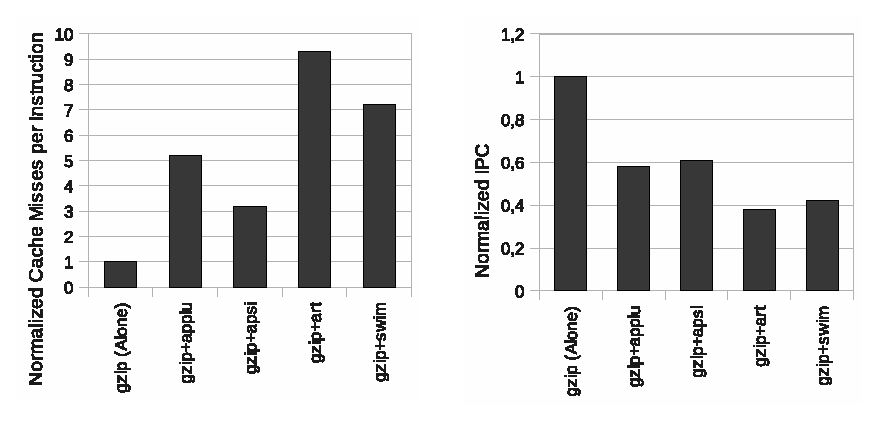
\includegraphics[width=\widefigure]{images/chandra_gzip}
\caption{\figurecaption{gzip miss rate}}
\label{fig:gzip_miss}
\end{figure}

The picture shows gzip's number of cache misses per instruction and instruction per cycle (IPC), when it runs alone compared to when it is
co-scheduled with different threads, such as applu, apsi, art, and swim. All the bars are normalized to the case where gzip is running alone.
It is interesting to note how gzip's number of cache misses per instruction increases significantly compared to when it runs alone. Infact, it increases 
by 3x when it runs with apsi and by 9.5x when it runs with art, 7.3x when it runs with swim.
Consequently, the IPC is affected differently. It is reduced by 35$\%$ when gzip runs with apsi, but reduced by 63$\%$ when gzip runs with art. 
Although not shown in the figure, art, apsi, applu, and swim's cache miss per instruction increases less than 15$\%$ when each of them runs with gzip. 

In terms of fairness, gzip's significant slow down can easily result in \textbf{priority reduction}. 
For example, if gzip has a higher priority than art, for gzip to achieve a higher progress rate, it has to be assigned more than three times the 
number of time slices compared to that assigned to art. Otherwise, to the end users, gzip may appear to be starved. In terms of throughput,
gzip's significant slow down reduces the overall throughput because the utilization of the processor where gzip runs on is also significantly reduced. 
Furthermore, it is possible that the co-scheduled threads's working sets severely overflow the cache and create a \textit{trashing} condition.

In briefly, there are at least three problems that may happen and render the OS schedule ineffective.
The first problem is \textit{thread starvation}, which happens when one thread fails in competing for sufficient cache space necessary to make 
satisfactory forward progress. The second problem is \textit{priority reduction}, where a higher priority thread achieves a slower forward
progress than a lower priority thread, despite the attempt by the OS to provide more timeslices to the higher priority thread. It's as if the higher 
priority task and lower priority task have the same priority, that is the priority of higher priority task is reduced.
This happens when the higher priority thread loses to the lower priority thread (or other threads) in dealing for cache space. 
To make things worse, the operating system is not aware of this problem, and hence cannot correct this situation (by assigning more timeslices to the 
higher priority thread). The third problem is that the forward progress rate of a thread is \textit{highly dependent} on the thread mix in a co-schedule. 
This makes the forward progress rate difficult to characterize or predict, making the system behavior unpredictable. Unfortunately, despite these problems, 
cache implementations today are thread-blind, producing unfair cache sharing in many cases.

As I said in the first chapter, in these years were developed some ideas about how to make a scheduler cache-aware.
This chapter aims to show the general structure and strategies used to model cache behaviour followed by these algortihms, that are the most interesting 
part of these type of heuristics.

%%%%%%%%%%%%%%%%%%%%%%%%%%%%%%%%%%%%%%%%%%%%%%%%%%%%%%%%%%%%%%%%%%%%%%%%%%%%%
\section{Survey on cache architecture}
\label{sec:s1}

Over the years, cache architectures have always played an important role in system performance. Hundreds of research papers show how performance
can be improved using multi-level caches on a single-processor machine. Multicore systems introduce new challenges for cache designer, because cache memory 
is a shared resource, therefore issues related to how a core access to cached data and how the coherence regarding the access from different processors 
to the same cached data is guaranteed are unavoidable. Furthermore, caches play an important role in management of communication between different core.
This section aims to show which are most important factors introduced in cache architecture to take in consideration during the development of cache aware
algorithms from scratch. These cache characteristics are common in both general purpose and embedded systems.

%-----------------------------------------------------------------------------
\subsection{Cache coherent protocols}

Usually in multicore architecture, there is a private L1 cache for each core, and there is a L2 or L3 cache shared among all cores (SMP), or among cores 
that belong to the same node (NUMA). Shared cache is one of the most critical resources in multicores.

As for all types of shared resources, also for shared cache it's necessary to ensure integrity of the shared data.
When two or more CPUs operate on a shared variable and one of these CPUs modify the variable, it is necessary that the information regarding
this change of value be communicated to the other CPUs. The mean used to communicate these informations is called \textit{coherence protocol}, it defines 
the rules used to comunicate memory update between different cores. Existing coherence protocols are classified based on the mechanism by which they ensure 
cache coherence: 

\begin{itemize}

\item Snooping based protocols: Each cache monitors address lines of shared bus for every memory transaction made by remote processors. Appropriate action
is undertaken when data locally cached is modified by this transaction, for example: a write by a remote processor into a data address locally cached 
results in an invalidation of the local cache copy.

\item Snarfing based protocols: A cache controller watches both address and data in an attempt to update its own copy of a memory location when a second 
master modifies a location in main memory. When a write operation is observed to a location that a cache has a copy of, the cache controller updates its 
own copy of the snarfed memory location with the new data.

\item Directory-based protocols: Shared data are placed in a common directory that maintains the coherence between processor caches. 
This directory acts as a look-up table for every processor to verify coherence of data that is currently being read or updated.

\end{itemize}


The first two mechanisms are typical of the SMP architecture, while the last is used in large point-to-point inter-processor communication network 
architectures. Snooping protocols became popular and widely accepted with multiprocessors systems since it required minimal change to the pre-existing 
physical shared bus interface to the memory. The inherent broadcasting property of the snoop protocols makes it simple to implement but places an upper 
limit on scalability.
Over the years, several snooping based cache coherence protocols were developed. The most common is MESI protocol.
With this protocol, every cache line is marked with one of the following states:

\begin{itemize}

\item Modified
The cache line is present only in one of the local caches, and it has been modified from the value in main memory. Write on a modified cache line are 
allowed, reads are a bit complicated. The local cache that owns a modified cache line must intercept (snoop) all attempted reads (from all of the other 
caches in the system) at main memory location that correspond to modified cache line, forcing them to back off, then writing data to main memory and change
state of cache line to shared state.
 
\item Exclusive
The cache line is present only in the current cache, and it matches main memory. It is possible to read/write lines in this state. A cache that owns
lines in exclusive state must snoop only all read transactions from all other cache and if it intercepts some read that regards owned cache line, it changes
the state of that line from exclusive to shared.

\item Shared
Indicates that this cache line may be stored in other caches and it matches the main memory. It is possible read cache line in this state. Writes to a 
shared cache line are allowed but before to perform the operation, it is necessary invalidate all other copies in other caches.
A cache that holds a line in the Shared state must listen for invalidation from other caches, and discard the line (by moving it into Invalid state) on a 
match.

\item Invalid
Indicates that this cache line is invalid, read/write operation on invalid cache line are denied

\end{itemize}

Cache coherence protocols play an important role to improve efficiency of the read/write in cache. There are a lot of variant of MESI protocol, the most 
recent variants are MESIF and MOESI.

The former protocol adds the Forward state. This state indicates that only one cache should act as a designated 
responder for any requests for the given line. With the standard MESI protocol, a request for cache line will receive a response from each cache that 
contains that line in the shared state. Instead, with MESIF protocol a request will be responded to only by the cache holding the line in the Forward state.
A cache line shared among multiple processors will be in Forward state in only one L3 cache. This protocol is used in new Intel microarchitecture Nehalem 
and it is designed for NUMA. The aim of this new state is to reduce communications between cache.

The latter protocol add Owned state. A cache line in this state holds the most recent, correct copy of the data. Only one processor can hold the data 
in the Owned state, all other processors that contains a copy of that data must hold the them in the shared state. A copy of data in main memory can be 
incorrect. A cache line in owned state may be changed to the Modified state after invalidating all shared copies, or changed to the Shared state by 
writing the modifications back to main memory, furthermore cache lines must respond to a snoop request with data. 
It is clear that the aim of this protocol is to avoid the need to write a dirty cache line back to main memory when another processor tries to read it. 
With the Owned state, processor can supply the modified data directly to the other processor. This is beneficial when the communication latency and 
bandwidth between two CPUs is significantly better than to main memory. An example of MOESI implementation is present in AMD Shanghai microprocessor.

%-----------------------------------------------------------------------------
\subsection{Inclusive and exclusive cache}

Another important architecture detail that affect performance is if a cache is inclusive or exclusive.
An inclusive cache means that all data available in higher level caches are contained also in the last level cache, namely in shared cache.
An exclusive cache means that data is present only in one cache.

It is clear that these two architectural policies are focused on two different aspects. The first policy greatly reduces snoop traffic because if a core 
doesn't find requested data in any of its cache level, it knows the data it is also not present in any other core's cache. The second policy, instead, 
allows to store more data than an inclusive cache, because for each data only one copy is stored.

An example of inclusive L3 shared cache is implemented in Intel Nehalem microarchitecture. Each cache line in the L3 contains additional "core valid" bits,
one for each core in the system, denoting which cores may have a copy of that line in their private caches. If a "core valid" bit is set to 0, then that 
core cannot possibly have a copy of the cache line, while a "core valid" bit set to 1 indicates it is possible (but not guaranteed) that the core in 
question could have a private copy of the line. Since Nehalem uses the MESIF cache coherency protocol, if a cache line in L3 have more than one 
"core valid" bits set to 1, the cache line is guaranteed to be clean and it will be in Forward state in L3, in this way, the L3 is the only
responder for all request for that line. This greatly reduces the amount of traditional "snooping" coherency traffic between cores.

An implementation of exclusive cache can be found in AMD's Shanghai processors. Theese cpus present an interesting implementation of this type of cache
architecture, because L1 and L2 are exclusive cache, but last level shared cache (L3) is a not-inclusive cache.
Not-inclusive architecture is a variant of exclusive architecture, becasue if a cache line is transferred from the L3 cache into the L1 of any core, the 
line can be removed from the L3. According to AMD this happens if it is "likely" that the line is only used by one core, otherwise a copy can be kept in 
the L3. About how the cpu can "understand" if a line will be used only by one core, AMD has not revealed details. Nowadays, an inclusive cache is 
preferred over an exclusive cache, because it simplifies the problem of cache coherence. 

\begin{figure}[htbp]
\centering
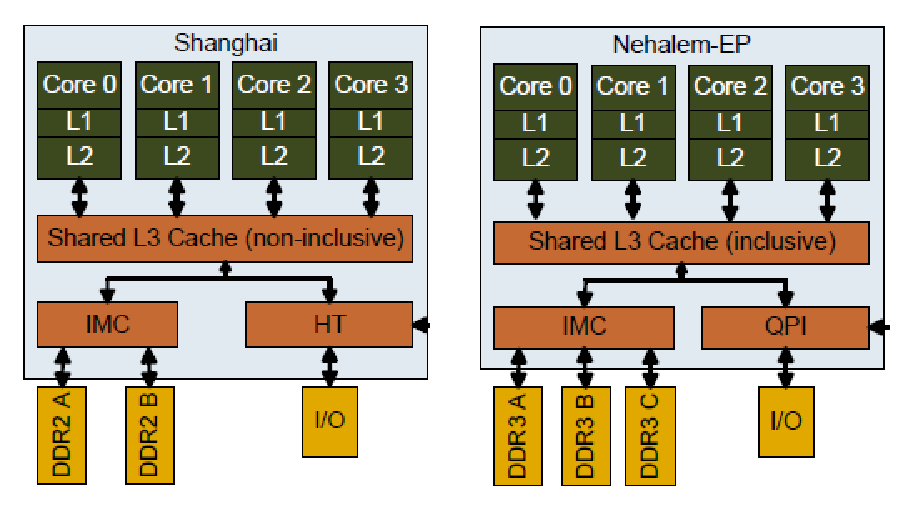
\includegraphics[width=\widefigure]{images/neh_amd.eps}
\caption{\figurecaption{AMD Shanghai and Intel Nehalem}}
\label{fig:neh_amd}
\end{figure}

To get a sense of how cache coherence impacts on system performance, it is possible to look over the work made by 
Molka et al. \cite{molka}. They have compared perfomance of MESIF protocol applied to inclusive cache (Intel Xeon 55** Nehalem) and MOESI protocol applied 
to an exclusive cache (AMD Shanghai), see figure \ref{fig:neh_amd}. These processors tested are multithreaded and ccNUMA dual-socket SMP systems. 
In the table \ref{fig:tab_lat} read latencies recorded during test are showed.

\begin{figure}[htbp]
\centering
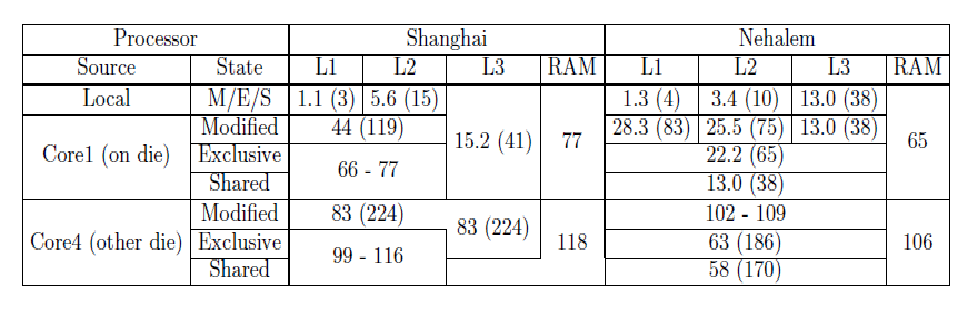
\includegraphics[width=\widefigure]{images/tab_lat.eps}
\caption{\figurecaption{read latencies}}
\label{fig:tab_lat}
\end{figure}

\begin{description} % off - on chip

\item[on-chip latencies] These data measure access time to the cache of other cores on the same die. We will see that having an inclusive cache or not
influence strongly this type of latency. 

\textbf{Nehalem:} A \textit{Shared} cache line in L3 is guaranted to be valid and it could be in shared or forward state, it can be accessed within 13 ns. 
An \textit{Exclusive} cache line that has core valid bit set in L3, may has been modified in higher level cache, this fact forces the L3 cache to check the 
coherency state in the core, therefore the latency increase up to 22.2 ns, furthermore, in the this type of cache, exclusive cache lines can be silently 
evicted from higher level cache and remain only in L3. The check on coherency state is made also for theese lines that are only in L3 cache.
A read of \textit{Modified} cache line present in other on-chip L1/L2 requires 25.5/28.3 ns, but if a modified line is evicted from L1/L2, it is required a 
write-back in L3 and an update of the core valid bits. It means that future access at that line will has a latency of 13 ns again.

\textbf{Shanghai:} A \textit{Shared or Exclusive} cache lines from higher level caches need to be fetched from the cores or main memory if no copy exists 
in the non-inclusive L3 cache. Latency showed in the table indicate that request for lines in theese state are serviced by main memory.
A \textit{Modified} state it's the only state that allow to avoid access to main memory.

\item[off-chip latencies] Theese data measure access time to the cache of other cores on another die. Theese latencies include additional penalty for the
QPI/HT data transfer. We will see that cache coherence protocol influence this type of latencies.

\textbf{Nehalem:} Thanks to inclusive cache, the access to unmodified data is fast. Latency for \textit{Exclusive} cache line include a snoop of one core 
(63 ns), \textit{Shared} cache line don't require snoop (58 ns). Moreover, latency for \textit{Modified} lines is higher (> 100 ns), becasue the MESIF 
protocol requires a write back to the main memory.

\textbf{Shanghai:} Cache lines in \textit{Shared} state are fetched from main memory (> 99 ns), L3 can satisfies request for \textit{Exclusive} cache lines 
(83 ns). Cache line in \textit{Modified} state can be forwarded to the requesting core from all cache levels, furthermore, thanks to MOESI protocol, a 
modified cache line in the remote cache can switch to the Owned state and avoid to be written back to main memory.

\end{description} % end on - off chip

It is intersting to note how  accesses to remote caches on Shanghai are slower than accesses to the local RAM (83 vs. 77 ns). 

%-----------------------------------------------------------------------------
\subsection{Cache Hardware prefetcher}

Finally, it is necessary to spend a few words about prefetching. Prefetcher is an hardware component that tries to predict which memory addresses are
going to be used by the program, in order to load needed data in cache memory.
Typical technical workloads often access memory in regular and sequential patterns, therefore, with a smart prediction mechanism, a prefetcher can select 
and preload correct data and, in this way, reduce memory latency. The key point to build a good prefetcher is to design prediction mechanism.
In literature there are many ideas to solve this problem. An example of concrete solution is the Intel Smart Memory access. This system was introduced
with Intel Core microarchitecture. In this system there are two prefetchers to the Level 1 data cache and the traditional prefetcher to the Level 1 
instruction cache. In addition there are two prefetchers associated with the Level 2 cache. In total, there are eight prefetchers per dual-core processor. 
In order to improve the accuracy of the prediction, the prefetcher system tags the history of each load using the Instruction Pointer (IP) of the load. 
For each load, the prefetcher builds a history and keeps it in a suitable history array. Based on load history, the prefetcher tries to predict the 
address of next load accordingly to a constant stride calculation (a fixed distance or "stride" between subsequent accesses to the same memory area). 
At this point, the prefetcher generates a prefetch request with the predicted address and brings the resulting data to the Level 1 data cache.
In literature, this kind of prefetchers are called \textit{strided} prefetcher.
Other architectures, such as Power ISA\_2.06, that use a strided prefetcher, introduces cache instructions to hint prefetch system for data prefetching.
With this instructions an application can specify direction, depth, no of units and so on. In this way, the programmer has a low level control on 
data prefetched.

Another category of prefetcher are \textit{non-strided} data prefetcher. They are very useful for accessing complex and irregular data structures as 
linked list, B-Trees etc. There are different techniques to implement theese prefetcher, one of theese is "pattern history based prefetcher". 
In this approach, the prefetcher tracks the addresses of misses and tries to identify specific patterns of misses that occur together. 
Once a pattern of misses has been detected, the prefetcher will find the first miss in the pattern. When this first miss occurs again, the prefetcher 
will immediately prefetch the rest of the pattern. For traversing a complex data structure like a linked list, this would be a fairly effective approach.
Recently AMD has announced that it will employs a non-strided prefetcher in its brand new Bulldozer microarchitecture, but it has not revealed details on 
implementations.

%%%%%%%%%%%%%%%%%%%%%%%%%%%%%%%%%%%%%%%%%%%%%%%%%%%%%%%%%%%%%%%%%%
\section{Classification of cache-aware Scheduling algorithms}

Cache aware scheduling policies can be classified according to type of strategy followed. They are divided in \textit{data locality} and 
\textit{temporal locality} policies. The former type is focused on a smart allocation of resources in cache. These policies partition cache memory in order
to every task may use a dedicated area in cache memory and then, reduce inter-thread cache interference and miss rate.
The latter type is focused on cache reusability. These policies schedule tasks that subsequently will access at the same data, reducing miss rate.

%-----------------------------------------------------------------------------
\subsection{Data locality policies} 

These policies are focused on the use of Last Level shared Cache (LLC) made by scheduled tasks. They can be used both for Real-time and Fair tasks. 
They don't take care about core-local cache (usually L1) or other shared resources like interconnects. In literature, data locality is the most developed 
type of cache aware policies, because they can be integrated in every OS and are relatively simple policies to develop. Now I will show two examples of 
data locality policies and how they are implemented.

\begin{description}
\item[Cache aware Fixed priority policy:] To understand this type of policy assume this situation: consider a multicore platform consisting of $M$ cores 
with an on-chip LLC, and a task set $\tau$, in which each task $T$ releases a thread $J_i$ every period $p(T)$. Every released thread is characterized by a 
worst-case execution time (WCET) denoted by $C(T)$. It means that each thread released by task $T$ has a maximum duration of $C(T)$. For each thread is 
defined the number $A(J_k)$ that represents the total cache space size used by it: we define this space as per-thread \textit{working set sizes} (WSS). 
For simiplicity we assume that each thread generated by a task $T$ use the same number of partition, therefore it is possible to express $A(J_k)$ as $A(T)$. 
The quantity $e(T)/p(T)$ is called the utilization of $T$, denoted $u(T)$. The deadline $d(J_k)$ of a thread $J_k$ coincides with the release time of thread 
$J_{k+1}$. If thread $J_k$ completes its execution after time $d(J_k)$, then it is \textbf{tardy}. For some scheduling algorithms, tardiness may be bounded 
by some amount $B$, meaning that any thread $J_k$ will complete execution no later than time $d(J_k)+B$. Finally, assume that tasks have fixed priority.
This model describes very well a typical Real-time application.

A thread $J_k$ is scheduled for execution if:

\begin{enumerate}
	\item $J_k$ is the thread of highest priority among all waiting threads,
	\item There is at least one core idle
	\item There is enough cache space, i.e. at least $A(J_k)$ , is available.
\end{enumerate}

\begin{table}[htbp]
\begin{center}
\begin{tabular}{l|c|c|c}
	\hline
	& $p(T)$ & $C(T)$ & $A(T)$ \\ \hline
	$T_1$ & 3 & 2 & 1 \\ \hline
	$T_2$ & 4 & 3 & 2 \\ \hline
	$T_3$ & 5 & 3 & 2 \\ \hline
	$T_4$ & 8 & 3 & 1 \\ 
	\hline
\end{tabular}
\caption{An example task set}
\label{tab:cache_task_set}
\end{center}
\end{table}

\begin{figure}[htbp]
\centering
{
\psfrag{J11}{$J_{1}^1$}
\psfrag{J12}{$J_{2}^1$}
\psfrag{J13}{$J_{3}^1$}
\psfrag{J14}{$J_{4}^1$}
\psfrag{J21}{$J_{1}^2$}
\psfrag{J23}{$J_{3}^2$}
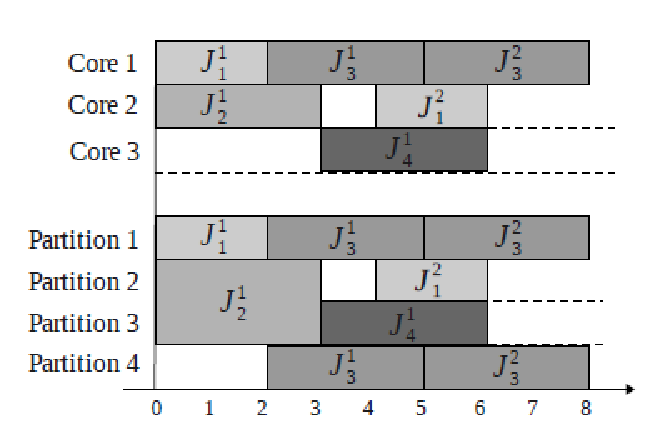
\includegraphics[width=\widefigure]{images/schedule.eps}
}
\caption{\figurecaption{Example of scheduling performed by cache aware policy}}
\label{fig:sched_example}
\end{figure}

Figure \ref{fig:sched_example} shows how the task set in Table \ref{tab:cache_task_set} is scheduled by the policy. The index of each task 
indentifies the task and indicates the priority of the latter. Higher priority is 1 and lower priority is 4. In the picture threads are represented in this 
way: $J_{\alpha}^\beta$, where $\alpha$ represents which task has released the thread, and then also its priority, and $\beta$ is an index that identifies 
the thread. We assume that co-scheduled threads use not-overlapped cache partitions.

At time 0 all threads are released. At this time, the thread $J_{4}^1$ can not be executed because it has lower priority than $J_{3}^1$ and the latter can 
not be scheduled since there is not enough idle cache partitions available.

It is clear that the aim of the described policy is to avoid cache trashing that occurs when the amount of space required by co-scheduled threads is greater 
than the dimension of LLC. A very important assumption made in this policy to achieve this goal is that all threads use not-overlapped 
partition of cache. This fact simplifies the scheduling problem, because it's enough to make a check on the amount of cache space occupied by co-scheduled 
threads to infer if cache thrasing occurs. Nevertheless, in practicei, this is not always true, because it greatly depends on type of application executed.


\textit{\textbf{Mechanisms and examples}} They key mechanism to reach this objective is profiler. At runtime, the profiler tries to infer what is the WSS 
of each scheduled task and provide these informations to scheduler. The challenge is how to do this thread. 
Calandrino et. al \cite{calandro} propose an interesting implementation of co-scheduler and for this type of policy.

The implementation is focused on Soft Real-time tasks, its solution is quite simple: it makes EDF cache-aware. Standard EDF algorithm gives higher priority 
to the task with earlier deadline in order to schedule it as soon as possibile. A cache-aware EDF is very similar to classic EDF: it "promotes", that is 
increases priority, of the thread with the smallest WSS, in this way threads on a runqueue are ordered by WSS.

The algortihm uses two separate run queues for eligible threads: the former is EDF-ordered, the latter is a "promotion" queue. In this queue, threads are ordered
from smallest to largest WSS. The thread in front of this queue is "promoted", that is its priority was increased and, for this reason, it remains at the front
of the queue and it will be the next task to execute. If there are tardy threads, they are inserted in EDF-ordered queue and they are scheduled according to 
EDF policy. The EDF-ordered queue contains task that have higher priority than tasks inserted in "promotion queue" TODO dai nomi a queste code.
When the heuristic picks a task from promotion queue, it checks if it will cause cache thrashing. For this reason, the scheduler mantains a variable with 
the total amount of the WSSs allocated, that is the cache space allocated. If this value plus the WSS of the thread to schedule exceeds the cache space size, 
thrashing will occur. In this case, the core remains idle and the thread waits for some thread that free cache resources.
Obiouvsly task priorities are respected, it means that a task with the smallest WSS is promoted only if it has the higer priority.

\begin{figure}[htbp]
\centering
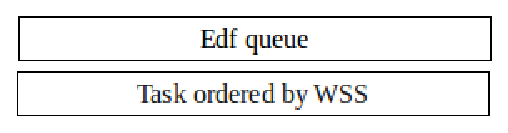
\includegraphics[width=\widefigure]{images/edf_wss.eps}
\caption{\figurecaption{queues used in the algorithm}}
\label{fig:edf_wss}
\end{figure}

To compute the WSS used by each task, the co-scheduler divides the total cache misses observed over all profiled threads by the total number of profiled 
threads, and multiplying the result by the cache line size. Cache misses and WSS are related, because, from experiments executed by Calandrino et al, 
follows that number of cache misses multiplied for dimension of a cache line gives a number proportional to WSS used by a thread. All the profiled threads 
belong to the same task. The co-scheduler discards measures obtained by threads that cause cache thrashing. Cache misses are recorded using performance 
counters. At the beginning of an application, there is not any measure about cache miss, therefore the profiler requires a bootstrapping phase in order to 
get necessary measures. This phase converge pretty fast to a reasonable result.

It is interesting to note, that in this implementation the only mean to avoid cache trashing is a check on amount of WSSs used by scheduled tasks.
This is a sub-optimal solution because cache trashing can occurs also in those cases where the total amount of WSSs is less than total amount of cache
space. To understand why, it is necessary to remind some consideration about cache architectures. When a cache miss occurs, it is necessary to make room 
in cache for the new entry to load. The heuristic that decide which is the entry to evict is called the replacement policy. According to replacement policy,
cache memory are classified in:

TODO img da mettere
\begin{description}
\item direct-mapped: a line in main memory can be placed only in one cache line. There is an 1:1 relationship between main memory and cache memory.
\item fully associative: a line in main memory can be placed in any cache line. There is a 1:N relationship between main memory and cache memory.
\item N-way set associative: it is a trade-off between direct-mapped and fully associative. Cache memory is divided in set, each set can contain N cache 
line. A line in main memory can be present only in one specific set and within it, that line can be placed in any line that belong to that set.
\end{description}

The reason is simple: the WSSs of two threads could be overlapped. It is very difficult in practice having not-overlapping WSS. Furthermore, also 
assuming true this hypotesis, 

TODO mettere le arch della cache

, furthermore, also under hypotesis of non-overlapped WSSs, check on WSS is sufficient
to prevent cache thrashing only if the cache is fully associative, because every line in main memory can be mapped on any cache line but, in a N-way 
set associative cache, a line in main memory can be mapped only within a certain set. For this reason, if a task occupies cache line used by a co-scheduled 


Considering this architecture detail, it is clear that check on WSS is sufficient to prevent cache thrashing only if the cache is fully associative, because every line in main memory can be mapped on any cache line but, in a N-way set associative cache, a line in main memory can be mapped only within a certain 
set. For this reason, if a task occupies cache line used by a co-scheduled task, cache trashing will occcurs. Furthermore, there is another important 
detail: we have assumed that non-overlapping WSS, but, in practice, this hypotesis is unlikely, therefore cache thrashing can occur also with a fully associative cache. Nervetheless, Calandrino et al. test their algorithm with Soft Real-Time multimedia application and, according to results showed 
\cite{calandro}, it seems that this sub-optimal solution is quite effective, at least with this kind of applications.

\textbf{\textit{Advantages and drawbacks}} This policy presents a clear drawback: it may waste resources. According to rules previously showed, if there 
is an idle core, but not enough cache space, a task may not be scheduled and, in this way, degrade throughput. 

Nevertheless, the policy improves predictability of the application, because, theoretically, each thread should find in cache enough space for its 
resources, mantaining constant its execution time. This aspect make this policy very indicate for Real-time system, where predictability is a very 
important aspect.

There is another important advantage related to improvement of predictability. On single-core systems there are well-developed techniques for timing 
analysis of embedded software. Using these techniques, the WCET of real-time tasks may be estimated, and then used for schedulability analysis. 
In multicore systems theese tecniques can't be used, because, as we have seen, cache behaviour (hit or miss) is unpredictable because it depends on which 
tasks are co-scheduled, therefore WCET can be variable and very difficult to estimate. With the analyzed policy, it is possible perform a proper cache 
isolation, that make cache behaviour more predictable and then it becomes feasible to execute a system-level schedulability analysis using existing WCET 
analysis techniques. For details on WCET analysis for Real-time system in multicore platform see \cite{guann}


\item[Fair cache sharing policy:]

This policy is focused on Fair tasks, therefore it considers an application model with less constraints than to that considered by
Calandrino et al. This implementation ensures \textit{fair cache sharing}, that is a strategy throughput oriented.

As we have previously seen, a bad combination of coscheduled tasks may cause cache thrashing and, consequently, a variation on task's instruction per cycle
(IPC) that determines task's performance variation. But, if co-scheduled tasks sharing cache in a fair way, they can allocate needed resources in cache and
they experience the fair IPC, that is the IPC that ensure the best overall performance. The mechanism used to ensure the fair IPC is to modify CPU timeslice 
assigned to a task, in this way, each task always run as quickly as it would under fair cache allocation, regardless of how the cache is actually allocated.

\begin{figure}[htbp]
\centering
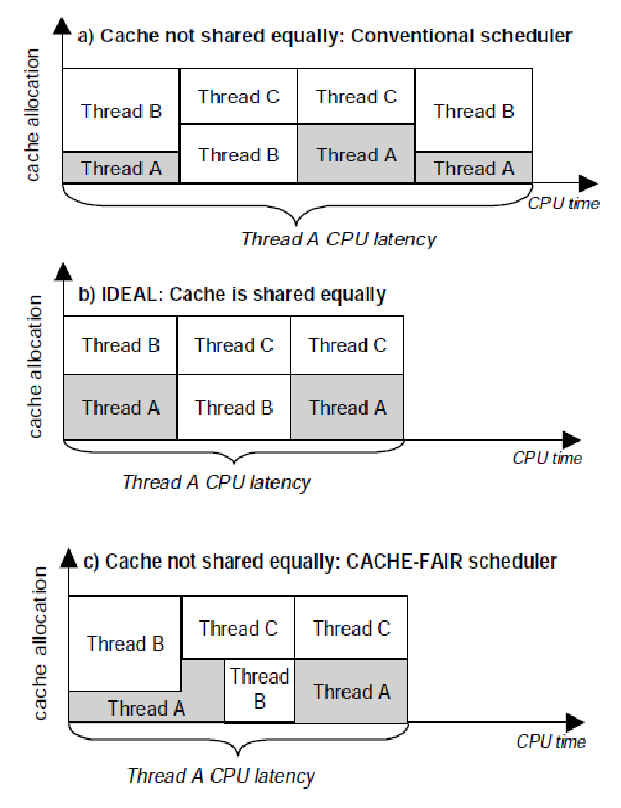
\includegraphics[width=\widefigure]{images/fed_cases.eps}
\caption{\figurecaption{queue used in the algorithm}}
\label{fig:fed_cases}
\end{figure}


In figure \ref{fig:fed_cases} is represented what the alorithm tries to do. Each box corresponds to a task. The height of the box indicates the amount of
cache allocated to the thread. The width of the box indicates the thread's CPU timeslice. The area of the box is proportional to the amount of work 
completed by the thread. Stacked thread boxes indicate corunners. In situation (a) is represented the ideal case, where all tasks share equally 
cache. In the case (b) is represented a real case where tasks don't share equally cache and, for this reason, Task A needs more CPU time to execute
all its job. Case (c) represents how is possible to ensure fair cache sharing: Task A can't make forward progress, so CPU timeslice of task A is increased 
and, at the same time it decreases timeslice of task B to mantain balanced CPU sharing. This is what the algorithm does. 


\textit{Mechanism and examples:} An implementation of this policy is developed by Fedorova et al. \cite{fedorova}. The algorithm is divided in two phases: 
sampling and scheduling. During the sampling phase, the co-scheduler gathers performance data and uses it to estimate the task's fair miss rate. During the 
scheduling phase, the scheduler periodically monitors the task's performance and adjusts the task's CPU timeslice if its actual performance deviates from 
its fair performance.

The fair miss rate and fair IPC of a task are estimated via performance counters, executing this experiment: different groups of corunners are formed, 
the task which we want to estimate fair miss rate is executed togheter to each group. At the end of execution, miss rates of each executed task are 
recored. Theese measures correspond to one data sample. It is necessary to collect at least ten data sample for each task, in order that each task has 
completed at least 100 million of instructions, to eliminate effects of compulsory misses. At the end of the sampling phase, the co-scheduler estimates the 
fair miss rate using a linear regression analysis and, according theese informations, also fair IPC is computed. In the scheduling phase, the scheduler 
monitors the task's IPC, again via performance counters. According to the difference between IPC measured and task's fair IPC, the scheduler adjusts task's 
CPU timeslice.

\begin{figure}[htbp]
\centering
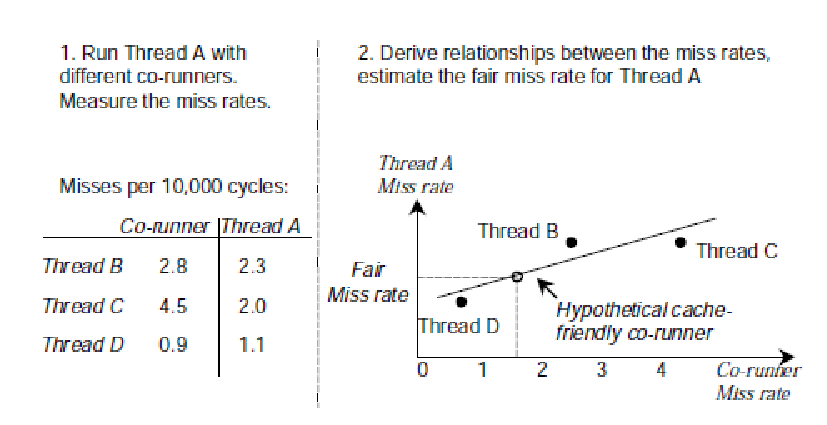
\includegraphics[width=\widefigure]{images/fedorova.eps}
\caption{\figurecaption{step of co-scheduler}}
\label{fig:fedorova}
\end{figure}


In Figure \ref{fig:fedorova} is reassumed how fair miss rate is estimated. Fedorova et al. found that that a linear function is the best approximation of 
relationship between co-runnners miss rates.

The overhead of sampling phase is fixed and it is repeated every time a thread has completed one billion instructions, while the check on a task's IPC
is made every 50 million instrucitons executed. When to check task's IPC and when to perform sampling phase is decided according to empirical observations
made by the developers of the algorithms.

It's important to note that this algorithm does not esablish a new CPU sharing policy but simply enforce existing policies. For example, if the 
system is using a fair-share policy, the cache-fair algorithm will make the cache-fair threads run as quickly as they would if the cache were shared 
equally, given the number of CPU cycles they are entitled to under the fair-share policy. Furthermore, the algorithm doesn't add any additional data 
strcuture, but simply requires only to record fair miss rate and fair IPC for each task.

\textbf{\textit{Advantages and drawbacks}}
Unlike previous example, this algorithm don't waste resource, moreover it use a more complex co-scheduler than that implemented by Calandrino et al, 
because it has to estimate fair miss rate of each task. According some statistical considerations, two corunner task experience fair cache sharing, if 
their miss rate is similar and that miss rate is the fair miss rate. To determine this value for each task, a possible approach consist of executing a task 
with all available corunner, but this approach is not feasible. The solution adopted by the co-scheduler, instead, consist of to run each task with a small 
number of possible corunner and use miss rates measured to derive a relationship between the miss rates of the task analyzed and its co-runners, and use 
that relationship to estimate task's fair miss rate. This procedure could introduce an higher unpredictability in the application and for this reason, that 
this algorithm couldn't be suitable for Real-Time systems, where predictability is required.

\end{description}

%-----------------------------------------------------------------------------
\subsection{Temporal locality policies} 

The idea behind this type of policies is very simple, but in practice it is more complex than the idea behind data locality policies. These policies 
require complex infrastructure and nowadays only few research activities have developed policies of this type. An interesting implementation of this type 
of policy can be found in COOL project \cite{COOL}. Recently Yang et al. \cite{taiwan} have implemented a scheduling algorithm inspired to these policies 
and naturally the concept of taskaffinity is a simplified implementation of temporal locality policies.

\begin{description}
\item[cache reusability policy]
The key point to maximize reusability of data in private cache, that is in L1 cache, is data sharing among tasks. If two threads, or in general two task, 
sharing common data, they are scheduled subsequently on the same cpu, in this way, it's more likely to reuse the same data in private cache.
According this observation, tasks are inserted in abstract list called \textit{sharing groups}. Tasks that share the same resources are put in the 
same sharing group. The scheduler assigns the same cpu at all tasks that are in the same sharing group, in this way they will use always the same private 
cache. 

Instead, to maximize reusability of data in shared cache, that is L2 or L3 cache, it is necessary to improve the opportunities that the subsequently 
scheduled tasks could reuse the data accessed by the current tasks at the scheduling point.

\begin{figure}[htbp]
\centering
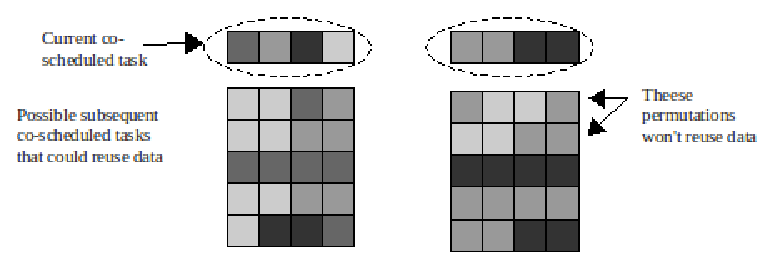
\includegraphics[width=\widefigure]{images/cosched_permutation.eps}
\caption{\figurecaption{task permutation}}
\label{fig:cosched_permutation}
\end{figure}


In figure \ref{fig:cosched_permutation} each square represents the data set used by a scheduled task, squares with different colours represent different 
data set. In case (a), four tasks are co-scheduled and they access to four different data sets. In the case (b) four co-scheduled tasks access to only two 
different data sets. To reuse the data in the cache, it is necessary schedule tasks that use data sets that have been accessed by current co-scheduled 
tasks subsequently. Therefore, more data sets are accessed by current co-scheduled tasks and there will be more opportunities that the subsequent 
coscheduled tasks could reuse the data in the shared cache. For example: in situation (a) there are $4^4$ permutations of co-scheduled tasks that could 
reuse the data, but only $2^4$ in situation (b). According this observation, the scheduler should schedule the tasks using as many data sets as possible, 
but at one important condition: the total amount of data set used by co-scheduled task, must be less than the total cache space, in order to avoid cache 
trashing.

The interesting thing, is that to maximize reuse of data present in private cache and to maximize reuse of data present in shared cache are not in conflict
with each other. The explanation is straightforward: each core executes a task that belongs to different sharing group, therefore co-scheduled tasks would 
access \textbf{different data sets}, in this way, the number of data sets accessed in shared cache is maximized.

According to this theory, it is possible to list the rules applied this kind of policy:

\begin{itemize}
	\item Co-schedule tasks that belong to different sharing groups. 
	\item Schedule a task only if it doesn't cause cache thrashing.
\end{itemize}

\textit{\textbf{Mechanism and examples:}} An implementation of this policy is developed by Yang et al. \cite{taiwan}. 

This implementation use an array of linked list. In each list are inserted tasks that sharing the same resources, for simplicity we call the $i-th$ list 
$SG_i$. Each list is characterized by total working set used by task inserted in, it is denoted with $TW_i$. It is clear that these list are the 
implementation of the sharing groups previously descibed, for this reason, from now I will call these lists sharing groups. Before to start, the algorithm 
assigns each sharing group to one cpu: if number of core (NC) is less than number of sharing groups (NS), a cpu will execute more than one sharing groups, 
see fig. \ref{fig:possible_cosched}.

\begin{figure}[htbp]
\centering
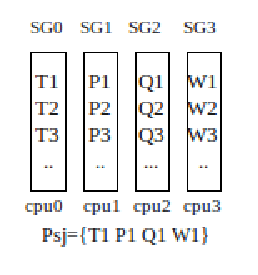
\includegraphics[width=\widefigure]{images/possible_cosched.eps}
\caption{\figurecaption{possible coschedule for a task j, in this case task A}}
\label{fig:possible_cosched}
\end{figure}

The heuristic is divided in two phases. In the first step, the algortihm chooses a task from each sharing group for a total of NC tasks, in this way, it
has defined a possible co-schedule ($PS_j$). It computes the sum of working set size (SWSS) of the $PS_j$ selected, if SWSS is greater than dimension of 
shared cache, $PS_j$ is discarded. This procedure is repeated for all possible $PS_j$. At the end, all filtered $PS_j$ that fit into the shared cache are 
put in a queue called $C$ and waiting for the next phase.

Before to analyze the next step, define the \textit{sharing number ($SC_j$)} as the number of different sharing groups belong to a possible filtered 
co-schedule $PS_j$. In the next step, elements present in queue $C$ are orderd according their $SC_j$. In order to schedule tasks that access the most 
different data sets, the algorithm select tasks that belong to $PS_j$ with the maximum $SC_j$.

If $C$ is empty, it means that there isn't any possible co-schedule $PS_j$ with the total working set size $TW_j$ that fit in shared cache. Also in this 
case, the algorithm would aim to minimize the shared cache misses by choosing the possible co-schedule with the maximum $SC_j$ and with smallest $TW_j$.

An interesting aspect of this implementation, is that it is possbile to reduce also cache coherence overhead, the reason is very simple. Tasks that belong 
to two different sharing groups don't share data, otherwise they should be in the same group. It means that lines used in private cache by
a co-scheduled tasks that are in different groups, won't never be in shared, but only in modfied or exlusive state. in this way, the overhead due to 
management of cache coherent shared state is reduced. 

Yang et al. implemented their algorithm in the scheduler present in Threading Building Blocks (TBB) that is a multrithreading library developed by Intel. 
This library allows to programmer to specify which is the working set of each threads and this information is just what it needs to implement their policy. 


\textbf{\textit{Advantages and drawbacks}}
This policy is an improvement of data locality policies, because, also in this case, it is essential to prevent cache trashing in LLC,
exploiting the same mechanisms used in data locality policies.

An important aspect of this policy is that it deals with cache coherence, that, as we have seen in previous section, is a very important factor that 
influence system performance. A drawback, is that to implement this policy is required an infrastructure that provide the same informations used in 
data locality policies, that is how much cache space a task use, and in addition, which are addresses used by task, that is a very difficult information
to obtain. To resolve this problem, the algorithm involves the programmer providing him a suitable API to influence the scheduling choices. This fact 
means to modify appllication code with additional functions. 
\end{description}

The difference between temporal locality policies data locality policies is very slight. The temporal locality policies, try to reduce cache misses 
choosing which tasks will be scheduled in two different moments. In other words, this type of policy, for each cpu, choose which task that will be 
scheduled after the current task in order that the next task will reuse resources already allocated in cache of each cpu. Instead data locality policies, 
try to reduce cache misses choosing tasks that cause the lowest inter task cache interference. In other words, this type of policy make sure that all 
scheduled task in the same moment may allocate necessary resources in shared cache.

